%
% File acl2015.tex
%
% Contact: car@ir.hit.edu.cn, gdzhou@suda.edu.cn
%%
%% Based on the style files for ACL-2014, which were, in turn,
%% Based on the style files for ACL-2013, which were, in turn,
%% Based on the style files for ACL-2012, which were, in turn,
%% based on the style files for ACL-2011, which were, in turn, 
%% based on the style files for ACL-2010, which were, in turn, 
%% based on the style files for ACL-IJCNLP-2009, which were, in turn,
%% based on the style files for EACL-2009 and IJCNLP-2008...

%% Based on the style files for EACL 2006 by 
%%e.agirre@ehu.es or Sergi.Balari@uab.es
%% and that of ACL 08 by Joakim Nivre and Noah Smith

\documentclass[11pt]{article}
\usepackage{acl2015}
\usepackage{times}
\usepackage{url}
\usepackage{latexsym}
\usepackage{graphicx}
\usepackage[]{algorithm2e}
\usepackage{amssymb}
\usepackage{amsmath}
\usepackage[inline]{enumitem}
\usepackage{color}
\usepackage{booktabs}
\newcommand{\tabitem}{~~\llap{\textbullet}~~}
\usepackage{array}
\usepackage{tabularx}

\DeclareMathOperator{\corpus}{\mathcal{C}}
\DeclareMathOperator{\doc}{\mathnormal{d}}
\DeclareMathOperator{\sent}{\mathnormal{s}}
\DeclareMathOperator{\order}{\pi}
\DeclareMathOperator{\dtime}{\mathnormal{t}}
\DeclareMathOperator{\hour}{\mathnormal{h}}
\DeclareMathOperator{\hours}{\mathcal{H}}
\DeclareMathOperator{\Sim}{\mathbf{K}}
\DeclareMathOperator{\SMat}{\mathbf{X}}
\DeclareMathOperator{\Pref}{\boldsymbol{\pi}}
\DeclareMathOperator{\Exemp}{\mathnormal{Exemplars}}
\DeclareMathOperator{\Updates}{\mathnormal{Updates}}


\newcommand{\query}[0]{q}
\newcommand{\stime}[0]{t_s}
\newcommand{\etime}[0]{t_e}

\newcommand{\fdadd}[1]{\textcolor{red}{#1}}
\newcommand{\fdcomment}[1]{\textbf{\textcolor{red}{[FD: #1]}}}
\newcommand{\ckcomment}[1]{\textbf{\textcolor{blue}{[CK: #1]}}}
\newcommand{\kmcomment}[1]{\textbf{\textcolor{green}{[KM: #1]}}}
\usepackage{titlesec}


%\titlespacing\section{0pt}{4pt plus 0pt minus 6pt}{4pt plus 0pt minus 4pt}
%\titlespacing\subsection{0pt}{4pt plus 0pt minus 6pt}{4pt plus 0pt minus 4pt}
%\titlespacing\subsubsection{0pt}{4pt plus 0pt minus 6pt}{4pt plus 0pt minus 4pt}
%\setlength\titlebox{5cm}

% You can expand the titlebox if you need extra space
% to show all the authors. Please do not make the titlebox
% smaller than 5cm (the original size); we will check this
% in the camera-ready version and ask you to change it back.


\newenvironment{blockquote}{%
  \par%
  \medskip
  \leftskip=1em\rightskip=1em%
  \noindent\ignorespaces}{%
  \par\medskip}

\title{Predicting Salient Updates for Disaster Summarization}

\author{Chris Kedzie \and Kathleen McKeown\\
Columbia University\\
Department of Computer Science\\
%  Affiliation / Address line 3 \\
{\tt \{kedzie, kathy\}@cs.columbia.edu} \\\And
%  Affiliation / Address line 1 \\
%  Affiliation / Address line 2 \\
%  Affiliation / Address line 3 \\
 Fernando Diaz\\
 Microsoft Research\\
  {\tt fdiaz@microsoft.com} \\ 
  }

\date{}

\begin{document}
\maketitle
\begin{abstract}
During crises such as natural disasters or other human tragedies, information
needs of both civilians and responders often require urgent, specialized
treatment.  
Monitoring and summarizing a text stream
during such an event remains a difficult problem. 
We present a system for update summarization which predicts the salience of 
sentences with respect to an event and then uses these
predictions to directly bias a clustering algorithm for sentence selection,
increasing the quality of the updates. We use novel, disaster-specific features
for salience prediction, including geo-locations and language models
representing the language of disaster.
Our evaluation on a standard set of retrospective events using ROUGE shows 
that salience prediction provides a significant improvement over 
other approaches.

\end{abstract}

\section{Introduction}

\section{Introduction}
\label{sec:introduction}
During crises, information is critical for first responders and those caught
in the event.  When the event is significant, as in the case of Hurricane
Sandy, the amount of information produced by traditional news outlets,
government agencies, relief organizations, and social media can vastly
overwhelm those trying to monitor the situation. Methods for identifying,
tracking, and summarizing events from text based input have been explored
extensively
%KM - I think we should consider adding other event summarizers. 
(e.g.,
\cite{allan1998topic,Filatova&Hatzivassiloglou.04a,Wang&al.11}). However,
these experiments were not developed to handle streaming data from  the large and heterogeneous
environment of the modern web. Neither were they developed to address the
information needs that arise during  crisis
situations. 
%KM - this last sentence sounds somewhat negative.
%there is still a need for robust and scalable 
%methods for automatic summarization.

In this paper, we present an update summarization system to track disasters
across time. Our system predicts sentence salience in the context of a
large-scale event, such as a disaster,  and integrates these predictions into
a clustering based multi-document summarization system. We train a regression
model to predict sentence salience and use these predictions to bias the
formation of sentence clusters around more salient regions in the input space
using affinity propagation (AP) clustering.  AP uses the salience predictions
as well as pairwise similarities among input sentences to identify
\emph{exemplar} sentences, which we use as our summary output.  Our approach
differs from other methods of summarization that compute salience by pairwise
comparisons alone, ignoring features of importance that are intrinsic to the
sentences themselves.

%KM - Chris - add a short overview on the kinds of things we measure and
%results so people are encouraged to read ahead. Keep it general.

In addition to the tight integration between clustering and salience
prediction, our approach also exploits knowledge about disaster to determine
salience. Thus, salience does not just represent importance within a set of
documents; it also represents both how typical this sentence is of the input event
type (i.e., disaster, hurricane, tornado) and whether it specifies information
about this particular disaster. We use a set of language models, one for each
disaster type, to measure typicality of the sentence for the current event type. We
use a feature that measures distance of mentioned location from the center of
the disaster to represent its likelihood of referring to the input disaster. 




%Previous work on generating event descriptions and/or multi-document
%summarization has relied on clustering algorithms to find representative
%sentences appropriate for an event summary.  These methods impose a metric
%space on the text data that can make it difficult to incorporate external
%sources of information elegantly -- in this paper we argue that centroid
%sentences are not a priori the best candidates for inclusion in an event
%summary.



The remainder of the paper is organized as follows. We begin with a review of related work in the information retrieval and multi-document summarization literature.  In section
~\ref{sec:background} we give an overview of the semantic similarity,
%KM - Chris can you update this so it reflects the contributions. We don't
%mention semantic similarity. We do mention salience and the disaster specific
%features. Perhaps we should mention the use of a new approach for semantic
%similarity? 
Gaussian process, and affinity propagation algorithms that make up the bulk of
our TS system. 
Next we describe the data with which we build our various models.
Then in section~\ref{sec:approach} we give a high level sketch
of our system, and then explain each component in detail. 


\section{Related Work}
\section{Related Work}
\label{sec:relatedwork}
A principal concern in extractive multi-document summarization is the
selection of salient sentences for inclusion in summary output
\cite{nenkova2012survey}.  This has often been approached as a ranking
problem.
%We broadly conceptualize this decision as either an intrinsic or extrinsic
%sentence evaluation process. Intrinsic approaches evaluate sentences
%individually, possibly by predicting the impact on summary quality using
%sentece level features. 
Sentences have been ranked by the average word probability, average tf-idf
score, and the number of topically related words (topic-signatures in the
summarization literature)
\cite{nenkova2005impact,hovy1998automated,lin2000automated}. The first two
statistics are easily computable from the input sentences, while the third
only requires an additional, generic background corpus.  Another ranking
approach, centroid summarization, involves creating an average bag of words
(BOW) vector, the centroid, from the input sentences and ranking sentences by
their similarity to the centroid \cite{radev2004centroid}.  Graph
\cite{erkan2004lexrank} and clustering
\cite{hatzivassiloglou2001simfinder,mckeown1999towards,siddharthan2004syntactic}
based approaches, on the other hand, make use of pair-wise similarity
comparisons amongst input sentences.  In these models, salient sentences are
more central to the input or cluster, respectively.

%identify salient regions of the input space while simultaneously coping with
%redundancy.  Graph-based algorithms have been used to rank sentences
%Clustering algorithms, e.g., are commonly used to exploit redundancy in
%input. Input sentences are clustered and summaries are generated by selecting
%the most representative sentence from each cluster.  Graph-based models have
%also been used for summarization.  E.g., the LexRank algorithm treats
%sentences as nodes in a graph, where edges are constructed by way of cosine
%similarity between sentence nodes; edges are either continuosly weighted by
%similarity or discrete, existing only when the similarity is above a
%threshold.  The PageRank algorithm is used on the graph to find the most
%important sentence nodes. In both clustering and graph-based approaches,
%sentence salience is largely determined by the pairwise relations between
%sentences.

Supervised learning has also been applied to this task. Model features are
usually derived from human generated summaries, and are non-lexical in nature
(e.g., sentence starting position, number of topic-signatures, number of
unique words, word frequencies). Seminal work in this area has employed naive
Bayes and logistic regression classifiers to identify sentences for summary
inclusion \cite{kupiec1995trainable,conroy2001using}. 

%\fdadd{
Several researchers have recognized the importance of summarization during
natural disasters.  Guo \textit{et al.} developed a system for detecting
novel, relevant, and comprehensive sentences immediately after a natural
disaster \cite{qi:temporal-summarization}.  The method uses a model of
sentence relevance and novelty in order to select appropriate updates.
Training data for regression targets is automatically generated from
retrospective Wikipedia data.  The system is evaluated on news documents
related to 197 natural and human disasters from 2009 to 2011 using variants of
Rouge modified to capture novelty, relevance, and comprehensiveness
\cite{lin2004rouge}.  Wang and Li present a clustering-based approach to
efficiency detect important updates during natural disasters
\cite{wang:update-summarization}.  The algorithm works by hierarchically
clustering sentences online, allowing the system to output a more expressive
narrative structure than Guo \textit{et al.}.  The method is evaluated on
official press releases related to Hurricane Wilma  in 2005 using Rouge score
between the system summary and a manually generated target summary.


\section{Method}

\section{Methods}

\subsection{Data}\label{sec:data}

Our primary datasets are the TREC 2013/2014 Stream Corpus, 
a ?tb corpus of hourly 
web crawls from October 2011
through mid February 2013 \cite{frank2012building}.\footnote{\url{http://trec-kba.org/kba-stream-corpus-2014.shtml}}
As per the TS specifications, all summary sentences come from processing this
corpus in a time aligned manner. While the 2014 corpus encompasses the 
2013 corpus, we use the 2013 corpus for evaluating events from the 2013 track
year because sentence ID's used in evaluation changed from year to year.

For our semantic similarity component (\cref{subsec:semsim}),
domain specific term-sentence matrices were built using subsections of
Wikipedia. For each event type we identified one or more related Wikipedia
categories and collected all pages that were listed under that category.
For all pages collected, we used the latest possible revision date before the
start of the Stream Corpus.

We use the same Wikipedia corpora to construct the lanuage models used
in our salience prediction model (\cref{subsubsec:lm}). 

\begin{figure*}
	\begin{center}
\begin{tabular}{| p{5cm} c c |}
\hline
Event & WP Categories & No. Docs/Sents/Words\\
\hline \hline
Boston\_Marathon\_bombings \newline
Christopher\_Dorner\_shootings\_and\_manhunt \newline 
 In\_Amenas\_hostage\_crisis
& Terrorism, Mass Shootings & 33,732/1,139,588/26,201,659  \\
\hline
 Cyclone\_Oswald \newline
Early\_2012\_European\_cold\_wave \newline
February\_2013\_noreaster \newline & Weather events & 35,554/591,850/12,794,438  \\
\hline
Costa\_Concordia\_disaster & Accidents & 22,874/732,945/16,520,242 \\
\hline
Chelyabinsk\_meteor & Earthquakes & 14,515/283,509/6,135,803  \\
\hline
Port\_Said\_Stadium\_riot \newline
2012\_Afghanistan\_Quran\_burning\_protests \newline
2011-13\_Russian\_protests \newline
2012\_Romanian\_protests \newline
2012-13\_Egyptian\_protests \newline
2013\_Bulgarian\_protests\_against\_the\_Borisov\_cabinet \newline
2013\_Shahbag\_protests & Activism\_by\_type & 464,657/11,254,122/250,172,896  \\
\hline
\end{tabular}
\caption{Domain specific Wikipedia corpora for semantic similarity and 
language models. }
\end{center}
\end{figure*} 

\subsubsection{Events}

We use the event set developed for the TREC Temporal Summarization track 
for years 2013 and 2014. There were 10 and 15 events respectively. We omit
one event from the 2013 track because there were no news documents in the 
corpus during the duration of the event, yielding a final event set of 24 
events. Meta-data provided for each event includes the name of the event
as it appears on Wikipedia, a short text query for the event, 
the type of event, and the 
duration of the event (the duration for the system 
to monitor not necessarily the complete timespan of the event). 
All data except the Wikipedia name is exposed to the TS system to use.  

\subsubsection{Nuggets}
For evaluation purposes, important pieces of information, hereafter 
referred to as nuggets, were extracted from each event's Wikipedia page.
Assessors graded nuggets by importance, and were also able to timestamp their
existance using the timestamp of the page's revision history. Nuggets are 
usually a short to medium length clause containing an atomic piece of
information.

\subsubsection{Matches}
TREC assessors provided judgements on a subset of participant updates each year
of the track. Judged updates are matched to one or more nuggets (a real 
sentence often contains more than one atomic piece of information) or marked
not relevant. There was not much overlap in the participant update sets so
overall coverage of relevant sentences in the corpus is small (percent?).
To expand the judgement corpora, we include all system updates as positive
nugget matches if they are $< .2$ close in Levenshtein distance to a human
assessed matched update. 

\subsection{Experiment Design}

\subsubsection{Salience Models}
For each event (both in the complete system and feature ablation experiments)
we randomly sample 1000 sentences after relevant document filtering and 
over the duration of the event 
(as determined by 
TREC; avg. run length is ? days) of the event. Nugget similarities
are computed for each sentence and are standardized with respect to 
the sample mean and variance. After standardization, the maximum nugget similarities are computed for each sentence. 
We fit a Gaussian process for each event, using the maximum similarities 
as our regression target, yielding 24 models in total. Kernel lengthscale
parameters are also individually fit for each model.
When making event-specific predictions, we take the average prediction of the
23 other models.

\subsubsection{Redundancy Threshold}

For every time interval with input, a clustering algorithm is
guarranteed to produce at least one output; 
this can significantly hurt the performance of all clustering based 
temporal summarization systems. In order to avoid this, we set a threshold $t$
such that a new update must have a maximum similarity $< t$ to all previous 
updates.

We determined the value of $t$ by examining the distribution of similarities
of nuggets to their human-matched sentences compared to the distribution
of similarities of nuggets to relevant but non matching sentences. We fit
normal distributions for the matching and non-matching similarities and
used the point of intersection as the value of $t$.
Figure ? shows a normalized histogram of cosine similarities for both 
distributions, the fitted distributions, and the point of intersection.

\begin{figure}
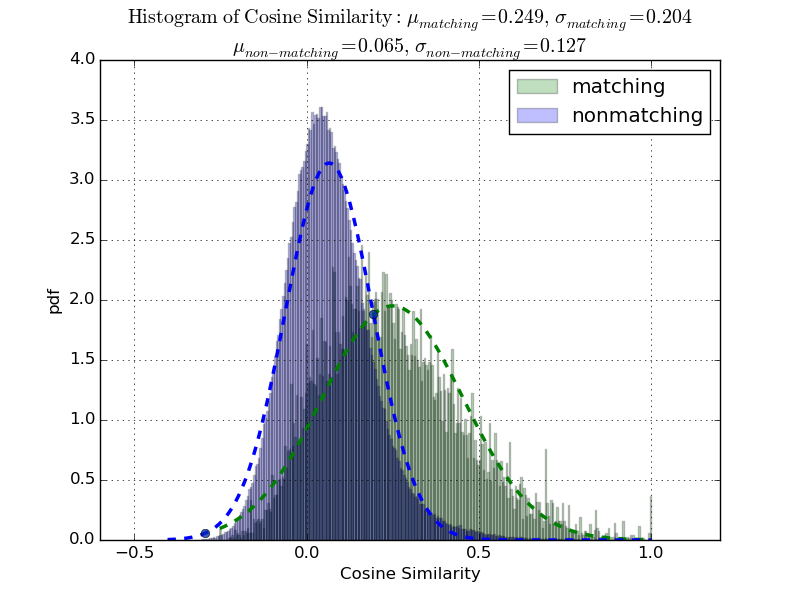
\includegraphics[scale=.40]{match-dist.png} 
\caption{Distribution of nugget similarity for matching and non-matching 
updates.}
\end{figure}
\subsubsection{Effect of Salience Models}

In order to assess the effectiveness of the salience predictions on update
selection, we perform a baseline (AP-base) run using affinity propagation 
clustering
with uniform preference, i.e. all preferences are equal to the median sentence
similarity. This run is compared to our full system (AP-sal), using each
sentence's salience prediction as its preference. 

We are also interested
in the effect of directly incorporating salience in the clustering algorithm.
A third run (HAC) is performed using hierarchical agglomerative 
clustering; we produce flattened clusters by setting a maximum cluster 
distance threshold. The sentence with the highest predicted salience from each
 cluster is selected as an update. 
The distance threshold was tuned using grid search. By comparing
HAV with AP-base we can empirically assess the trade off between preference
and neighbor similarity that affinity propagation is making.

\subsubsection{Feature Ablation}

We remove each feature group and train models models on these small faller 
feature susbstets. All other parameters are the same as in our full system 
(AP-sal).





\section{Data}
\label{sec:data}
For the document stream, we use the news portion of the
 2014 TREC KBA Stream Corpus.
The documents from this corpus come from hourly crawls of the web covering 
 October 2011 through February 2013. 


Our experiments also make use of the TREC Temporal Summarization (TS) Track
 data from 2013 and 2014 \cite{aslam2013trec}. 
This data includes 25 events and event metadata (e.g., a user
search query for the event, the event type, and event evaluation timeframe).  
All events occurred during the time span of the TREC KBA Stream Corpus.
For each event we create a stream of relevant documents by 
selecting only documents with article content that contains the complete set 
of query words. 
%identifying the 
%article start/end within each web page in the corpus using a classifier
%tra
%those documents

Along with the metadata, NIST assessors constructed a set of ground truth nuggets for each event. 
Nuggets are brief and important text snippets that represent sub-events that should be conveyed
by an ideal update summary. % (see Figure~\ref{fig:nuggets} for examples).
In order
to accomplish this, for each event, assessors were provided with the
revision history of the Wikipedia page associated with the event.  
For example, 
the revision history for the Wikipedia page for `Hurricane Sandy' will 
contain text additions including those related to individual nuggets.  The assessment
task involves reviewing the Wikipedia revisions in the evaluation timeframe 
and marking the text additions capturing a new, unique nugget.  More detail
on this process can be found in the track description \cite{aslam2013trec}.




\section{Experiments}
\label{sec:exper}
We evaluate our system on two metrics: ROUGE \cite{?}, a common automatic
summarization method and an evaluation of system expected gain 
and comprehensiveness---metrics adapted 
from the Trec TS track \cite{?}.


\subsection{Training and Testing}

Of the 25 events in the TREC TS data, 24 are covered by the news portion 
of the Trec KBA Stream Corpus.
From these 24, we set aside three events to use as a development set.
All system salience and similarity threshold parameters are tuned on the
development set.

We train a salience model for each event using 1000 sentences randomly sampled
from the event's document stream. Kernel length scale parameters  for each
feature group are fit to maximize
the model's log likelihood using ???.

We perform a leave-one-out evaluation of each event.
At test time, we predict a sentence's salience using the average predictions
of the 23 other models.   

\subsection{ROUGE Evaluation}

ROUGE measures the ngram overlap between a model (i.e. human) summary 
and an automatically generated system summary. 
Model summaries for each event were constructed by concatenating the event's 
nuggets. 
See figure~\ref{fig:test} for an example model summary excerpt.
Generally, ROUGE evaluation assumes both model and system summaries
are of a bounded length. Since our systems are summarizing events over a span
of two weeks time, the total length of our system output is much longer than
the model. To address this, for each system/event pair, we sample with replacement
1000 random summaries of length less than or equal to the model summary 
(truncating the last sentence when neccessary). The final ROUGE score for the 
system are the average scores from these 1000 samples.

Because we are interested in system performance over time, we also evaluate 
systems at 12 hour intervals using the same regime as above. 
The model summaries in this case are retrospective, 
and so we can see how quickly
each system is able to achieve its maximum performance.

\subsection{Expected Gain and Comprehensiveness}

NIST developed a series metrics for evaluating update summarization systems
as part of the TREC TS track.
We present results on two of these metrics, the expected gain and 
comprehensiveness.

\textbf{Expected Gain } We treat the event's nuggets as unique units of 
information.
When a system adds an update to its summary, it is potentially adding some
of this nugget information. It would be instructive to know how much unique
and novel information each update is adding on average to the summary.
To that end, we define

\[ \mathrm{\mathbb{E}[Gain]} = \frac{|S_n|}{|S|}% \;\;\; \mathrm{Recall} = \frac{|S_n|}{|N|}
\] 
where $S$ is the set of system updates, 
$S_n$ is the set of nuggets contained in $S$, and $|\cdot|$ is the number of
elements in the set.
To compute the set $S_n$ we match each system update to 0 or more nuggets, 
where an update matches a nugget if their semantic similarity is above 
a threshold. $S_n$ results from the unique set of nuggets matched.
Because an update can map to more than one nugget, it is possible to receive an
expected gain greater than 1; values greater than one can be thought of as a 
compression ration, i.e. an expected gain of 10 indicates the average update
contains 10 unique nuggets on average and that the summary is a 10~:~1 
compression of the nugget information.
An expected gain of 1 would indicate that every
sentence was both relevant and contained a unique piece of information.



\textbf{Comprehensiveness } Additionally, we can use the nuggets to measure the completeness of an update 
summary. We define

\[ \mathrm{Comprehensiveness} = \frac{|S_n|}{|N|}\]

where $N$ is the set of event nuggets.
A comprehensiveness of 1 indicates that the summary has cover 
all nugget information for the event; the maximum
attainable comprehensiveness is 1.

Update-nugget matches are computed automatically, where a
match exists if the semantic similarity of the update/nugget pair is above 
a threshold.
Determining an optimal threshold to count matches is difficult so 
we evaluate at 
threshold values ranging
from .5 to 1, where values closer to 1 are more conservative estimates of
performance.
A manual inspection of matches 
suggests that semantic similarity values around .7 produce reasonable matches.
For example, the nugget 
\begin{blockquote}
watches and warnings in effect for much of the Mid-Atlantic states and 
southern New England 
\end{blockquote}
\noindent
matches with the update 
\begin{blockquote}
A tropical storm warning remains in effect for much of the coasts 
of North and South Carolina\end{blockquote}
\noindent
with a similarity of .7. 
The average semantic similarity of manual matches performed 
by NIST assessors was considerably lower at approximately .25, increasing
our confidence in the automatic matches in the .5--1 range.


\subsection{Model Comparisons}
We refer to our complete model as \textbf{AP+Salience}.  We compare this model again several variants and baselines intended to measure the contribution of different components. All thresholds
for all runs are tuned on the development set.

\textbf{Affinity Propagation only (AP) } The purpose of this model
is to directly measure the effect of integrating salience and clustering by providing a baseline that uses the identical 
clustering component, but without the salience information.
In this model, input sentences are apriori equally likely to be exemplars;
%clustering algorithm without the salience predictions.
the salience values are uniformly set as the median value of the 
input similarity scores, as is commonly used in the AP literature \cite{?}.
After clustering a sentence batch, the exemplars are examined in order
of increasing time since event start and selected as updates if their
maximum similarity to the previous updates is less than $\lambda_{sim}$,
as in the novelty filtering stage of AP+Salience.

\textbf{Hierarchichal Agglomerative Clustering (HAC)} : We provide another clustering baseline, single-linkage hierarchichal agglomerative clustering.
We include this baseline to show that AP+Salience is not just an improvement
over AP but centrality driven methods in general.
HAC was chosen over other clustering approaches because the number of clusters 
is not an explicit hyper-parameter. To produce flat clusters from the hierarchical clustering, we flatten the HAC dendrogram
using the cophenetic distance criteria, i.e. observations in each flat cluster have no greater a cophenetic distance than a threshold.
Cluster centers are determined to be the sentence with highest cosine similariy to the flat cluster mean.
Cluster centers are examined in time order and are added to the summary if their similarity to previous updates is below a similarity threshold $\lambda_{sim}$ as is done in the AP model.

\textbf{Rank by Salience (RS)} 
We also isolate the impact of our salience model in order to demonstrate 
the that the fusion of clustering and salience prediction improves over
predicting salience alone.
In this model we predict the salience of sentences as in step 1 for 
AP+Salience. %However, rather than clustering, we simply rank the sentences
%by salience.
We omit the clustering phase (step 2).
Updates are selected identically to step 3 of AP+Salience, proceeding 
in order of decreasing salience, selecting updates that are above a salience 
threshold $\lambda_{sal}$ and below a similarity threshold $\lambda_{sim}$
with respect to the previously selected updates.


\fdcomment{consider removing AP+SalienceTR}
\textbf{AP+Salience Time Ranked (AP+SalienceTR)} Our final model is identical 
to the
AP+Salience model except at the novelty filter stage.
Within the novelty filtering stage, 
AP+Salience inspects exemplars in order of decreasing salience when computing
similarity to previous updates. Because the order in which we add updates
affects future similarity calculations, we evaluate an alternate ordering 
scheme (AP+SalienceTR) where exemplars are selected in order of increasing 
time since event start. The purpose of this model is to give preference to 
more recent updates, since timelyness is one of the desirable traits of our update
summaries.



\section{Results}
\label{sec:results}

\subsection{ROUGE}
\begin{table}[h]
\centering
% centering table
\begin{tabular}{l c c c}
% creating 10 columns
\multicolumn{4}{c}{ROUGE-1}\\
\hline
\hline
% inserting double-line
$\mathrm{System}$ & $\mathrm{Recall}$ & $\mathrm{Prec.}$ & $\mathrm{F}_1$\\
[0.5ex]
\hline
AP+Salience & $\mathbf{0.282}$ & $\mathbf{0.344}$ & $\mathbf{0.306}$ \\
AP          & $0.245$ & $0.285$ & $0.263$ \\
RS          & $0.230$ & $0.271$ & $0.247$ \\
HAC         & $0.169$ & $0.230$ & $0.186$ \\
\hline % inserts single-line
\end{tabular}
~\\[1ex]
~\\
\begin{tabular}{l c c c}
% creating 10 columns
\multicolumn{4}{c}{ROUGE-2}\\
\hline
\hline
% inserting double-line
$\mathrm{System}$ & $\mathrm{Recall}$ & $\mathrm{Prec.}$ & $\mathrm{F}_1$\\[0.5ex]
\hline
AP+Salience & $\mathbf{0.045}$ & $\mathbf{0.056}$ & $\mathbf{0.049}$ \\
AP          & $0.033$ & $0.038$ & $0.035$ \\
RS          & $0.031$ & $0.037$ & $0.034$ \\
HAC         & $0.017$ & $0.024$ & $0.019$ \\
\hline % inserts single-line
\end{tabular}
%~\\[1ex]
%~\\
%\begin{tabular}{l c c c}
%% creating 10 columns
%\multicolumn{4}{c}{ROUGE-L}\\
%\hline
%\hline
%% inserting double-line
%$\mathrm{System}$ & $\mathrm{Recall}$ & $\mathrm{Prec.}$ & $\mathrm{F}_1$\\[0.5ex]
%\hline
%AP+Salience & $0.275$ & $0.336$ & $0.299$ \\
%AP          & $0.241$ & $0.280$ & $0.258$ \\
%RS          & $0.225$ & $0.265$ & $0.242$ \\
%HAC         & $0.166$ & $0.225$ & $0.182$ \\
%\hline % inserts single-line
%\end{tabular}
%
%
\caption{System ROUGE performance.} % title name of the table
\label{tab:rouge}
\end{table}






Table~\ref{tab:rouge} shows our results for system output samples against the full summary of nuggets using ROUGE. 
%shows our results for the evaluation using ROUGE. 
%AP+Salience shows improvement on ngram precision and recall over the 
%baselines. 
This improvement is statistically significant for all ngram and longest common substring
precision, recall, and F-measure
at the $\alpha = .01$ level
using the Wilcoxon signed-rank test. 

\begin{figure}
    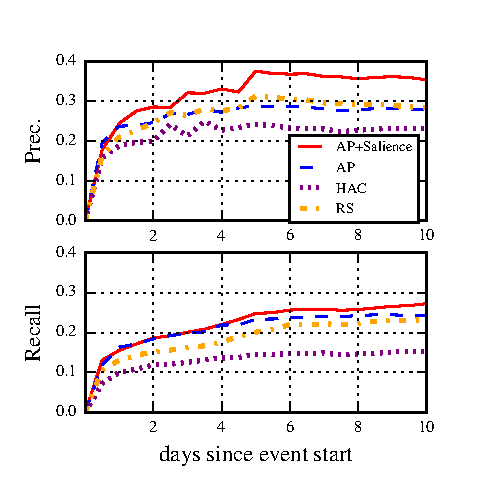
\includegraphics[]{rouge-time.eps}
\caption{System ROUGE-1 performance over time.}
\label{fig:trouge}
\end{figure}


AP+Salience maintains its performance above the baselines over time as well. Figure~\ref{fig:trouge}
shows the ROUGE-1 scores over time. 
We show the difference in unigram precision (bigram precision is not shown but it follows
similar curve).
Within the initial days of the event, AP+Salience is able to take the lead over the over 
systems in ngram precision. 
The AP+Salience model is better able to find salient updates
earlier on; for the disaster domain, this is an especially important quality of the model. 

Moreover, the AP+Salience's recall is not diminished by the high precision and remains competitive with AP.
Over time AP+Salience's recall also begins to pull away, while the other models start to suffer
from topic drift.


\subsection{Expected Gain and Comprehensiveness}
\begin{figure}
  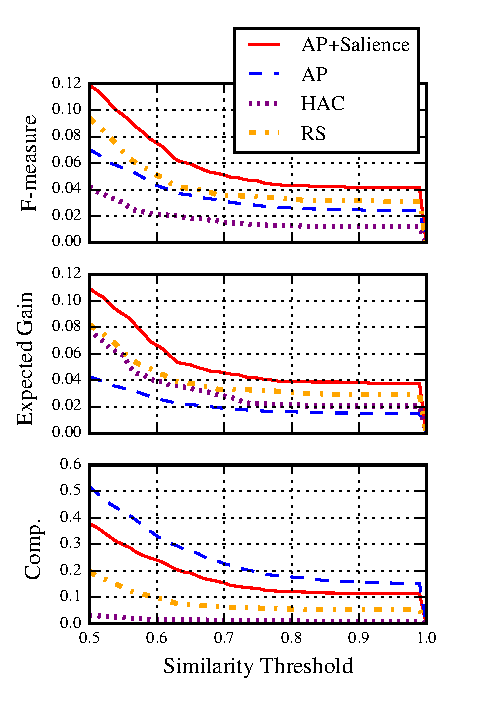
\includegraphics[]{nuggets-metrics.eps}
\caption{Expected Gain and Comprehensiveness performance.}
\label{fig:nperf}
\end{figure}

Figure~\ref{fig:nperf} shows the expected gain across a range of 
similarity thresholds, where thresholds closer to 1 are more conservative
estimates. The ranking of the systems remains constant across the 
sweep with 
AP+Salience beating all baseline systems.
Predicting salience in general is helpful for keeping a summary on topic as
the RS approach out performs the clustering only approaches
on expected gain.

When looking at the comprehensiveness of the summaries AP outperforms
 AP+Salience. The compromise encoded in the AP+Salience objective
function, between being representitive and being salient, is seen clearly here
where the performance of the AP+Salience methods is lower bounded by 
the salience focused RS
system and upper bounded by the clustering only AP system.
Overall, AP+Salience achieves the best balance of these two metrics.



\subsection{Feature Ablation}
\begin{table}[h]
\centering
% centering table
\begin{tabular}{l c c c}
% creating 10 columns
\multicolumn{4}{c}{ROUGE-1}\\
\hline
\hline
% inserting double-line
$\mathrm{System}$ & $\mathrm{Recall}$ & $\mathrm{Prec.}$ & $\mathrm{F}_1$\\
[0.5ex]
\hline
Full System & $0.282$ & $0.344$ & $0.306$ \\
No Basic    & $0.263$ & $0.380^\dagger$ & $0.294$ \\
No LM       & $0.223^\dagger$ & $0.361$ & $0.254^\dagger$ \\
No Time  & $0.297^\dagger$ & $0.367^{\dagger\dagger}$ & $0.322^\dagger$ \\ 
No Geo   & $0.232^{\dagger\dagger}$ & $0.381$ & $0.265^\dagger$ \\  
No Query & $0.251$ & $0.377$ & $0.280$ \\ 
\hline % inserts single-line
\end{tabular}
~\\[1ex]
~\\
\begin{tabular}{l c c c}
% creating 10 columns
\multicolumn{4}{c}{ROUGE-2}\\
\hline
\hline
% inserting double-line
$\mathrm{System}$ & $\mathrm{Recall}$ & $\mathrm{Prec.}$ & $\mathrm{F}_1$\\[0.5ex]
\hline
Full System & $0.045$ & $0.056$ & $0.049$ \\
No Basic    & $0.046$ & $0.068^{\dagger\dagger}$ & $0.051^\dagger$ \\
No LM       & $0.033^\dagger$ & $0.056$ & $0.038^\dagger$ \\
No Time  & $0.052^{\dagger\dagger}$ & $0.064^{\dagger\dagger}$ & $0.056^{\dagger\dagger}$ \\
No Geo   & $0.037^\dagger$ & $0.065$ & $0.042$ \\
No Query & $0.043$ & $0.068^\dagger$ & $0.048$ \\
\hline % inserts single-line
\end{tabular}
\caption{Feature ablation ROUGE performance. 
    $\dagger$ indicates statistically significant difference from 
full model at the $\alpha=.05$ level.
    $\dagger\dagger$ indicates statistically significant difference from 
full model at the $\alpha=.01$ level.
    } % title name of the table
\label{tab:farouge}
\end{table}








Table~\ref{tab:farouge} shows the results of our feature ablation
tests. Removing the language models yields a statistically 
significant drop in both ngram recall and F-measure. 
Interestingly, removing the basic features leads to an
increase in both unigram and bigram precision; in the bigram
case this is enough to cause a statistically significant increase
in F-measure over the full model. In other words, the generic features
actually lead to an inferior model when we can incorporate more appropriate
domain specific features.
This result mirrors Sparck Jones' claim that summarization should be in service of a purpose~\cite{?}.

Removing the language model and geographic relevance features leads to a
statistically significant drop in ROUGE-1 F1 scores. Unfortunately,
this is not the case for the temporal relevance features. We surmise that
these features are too strongly correlated with each other, 
i.e. the differences in TFIDF between hours are definitely not IID variables. 








\section{Conclusion}
In this paper, we have presented an update summarization system for the disaster domain,
and demonstrated improved system performance by integrating sentence salience with clustering.

Addtionally, we have shown that feature groups specifically targeted for the domain of disaster yield
better summaries; specifically features that capture the language and location
of the domain.


In the future we would like to explore the application of the AP+Salience
 model and features
%KM3 - I think not just for more general domains (as it says something wrong about this one) but to a wider class of events.
to a wider class of events. 

We would also like to further analyze the failure 
of the temporal relevance features; intuitively we believe time to be important
for the update summarization task.

%Addtionally we have presented several interesting feature groups for use in disaster summarization.
%In the future we would like to explore the applicability of this model and features
%to more general domains.


\section{Acknowledgments}

The research described here was supported in part by the National Science 
Foundation (NSF) under IIS-1422863. Any opinions, findings and conclusions or 
recommendations expressed in this paper are those of the authors and do not 
necessarily reflect the views of the NSF. 


% include your own bib file like this:
\bibliographystyle{acl} 
\bibliography{cites}

\end{document}
